% Chapter 3
\chapter{بررسی پیشینه روش‌های حل مشکل ناهمگنی آماری}

\section{مقدمه}
همان‌طور که در فصل گذشته اشاره شد، یکی از مهم‌ترین مشکلات در حوزه یادگیری فدرال، مسئله داده‌های غیرمستقل و غیریکنواخت
\lr{(non-IID)}
است که منجر به بروز چالش‌ها و ناهمگنی‌های آماری می‌شود. این مشکل باعث می‌شود که مدل‌های یادگیری نتوانند به خوبی از داده‌های توزیع‌شده استفاده کنند و کارایی مطلوبی داشته باشند. به دلیل اهمیت بالای این موضوع، محققان بسیاری تلاش‌های گسترده‌ای برای حل این مشکل انجام داده‌اند.

مبحث اصلی این پایان‌نامه نیز به طور دقیق به همین مسئله اشاره دارد و به دنبال یافتن راه‌حلی مؤثر برای مقابله با داده‌های
\lr{non-IID}
است. در ادامه، به صورت خلاصه به بررسی راه‌حل‌هایی که تاکنون برای حل این مشکل مطرح شده‌اند، خواهیم پرداخت تا تصویر جامعی از تلاش‌های انجام شده در این زمینه ارائه دهیم. همچنین باید توجه داشت که هر یک از این راه‌حل‌ها نقاط قوت و ضعف خاص خود را دارند و بسته به شرایط و نوع داده‌ها، می‌توانند نتایج متفاوتی را به همراه داشته باشند. بررسی دقیق این راه‌حل‌ها و ارزیابی کارایی آن‌ها می‌تواند به بهبود سیستم‌های یادگیری فدرال و غلبه بر مشکلات مرتبط با داده‌های غیرمستقل و غیر یکنواخت کمک شایانی کند.

\section{نگرش برپایه داده}
\subsection{اشتراک‌گذاری داده}
مشکل اصلی الگوریتم
\lr{FedAvg}
در مواجهه با داده‌های غیرمستقل و غیریکنواخت، تفاوت وزن‌های اولیه در شروع فرآیند آموزش است. این تفاوت‌ها می‌توانند باعث شوند که مدل‌های محلی در هر گره به طور قابل توجهی متفاوت از یکدیگر باشند، که در نتیجه منجر به مشکلات همگرایی و کاهش کارایی مدل نهایی می‌شود.

برای رفع این مشکل، روشی پیشنهاد شده است که در آن ابتدا سرور مرکزی مقدار کمی از داده‌ها را به صورت محلی آموزش می‌دهد. در این مرحله، سرور مرکزی با استفاده از این داده‌ها، یک مدل اولیه را آموزش داده و وزن‌های اولیه آن را تنظیم می‌کند. سپس، این وزن‌های اولیه به همراه داده‌های آموزش دیده شده به تمامی کاربران ارسال می‌شود. این اقدام باعث می‌شود که تمام کاربران در ابتدای فرآیند آموزش با مجموعه‌ای از داده‌های مشترک و وزن‌های اولیه مشابه روبه‌رو شوند.

نقطه قوت این روش در این است که به دلیل انجام این عملیات تنها در آغاز فرآیند آموزش، هزینه زیادی به شبکه تحمیل نمی‌شود. در واقع، انتقال داده‌ها و وزن‌ها فقط در ابتدا انجام شده و پس از آن کاربران به صورت مستقل به آموزش مدل‌های محلی خود ادامه می‌دهند. این اقدام منجر به کاهش اختلافات ناشی از ناهمگنی داده‌ها شده و فرآیند همگرایی مدل نهایی سریع‌تر و با دقت بیشتری انجام می‌شود
\cite{zhao2018federated}.

در شکل
\ref{share_data}%
، نحوه اجرای این روش و مراحل مختلف آن به تصویر کشیده شده است. این تصویر نشان می‌دهد که چگونه سرور مرکزی ابتدا داده‌های کمی را آموزش می‌دهد، وزن‌های اولیه را تنظیم می‌کند و سپس این وزن‌ها و داده‌ها را به کاربران ارسال می‌کند تا فرآیند آموزش محلی با یک نقطه شروع مشترک برای همه کاربران آغاز شود.

یکی دیگر از روش‌های مطرح شده در زمینه یادگیری فدرال به این صورت است که کاربران بتوانند نتایج آموزش تعدادی داده اشتراکی را با یکدیگر به اشتراک بگذارند و از نتایج دیگر کاربران بر روی این داده‌های اشتراکی مطلع شوند. در این روش، کاربران نتایج به‌دست آمده از آموزش داده‌های مشترک را با هم مبادله می‌کنند، که این کار منجر به بهبود عملکرد مدل‌های محلی و در نهایت مدل سراسری می‌شود
\cite{collins2021exploiting}.

براساس بررسی‌های انجام شده، مثلاً در مجموعه داده
\lr{CIFAR-10}،
اگر حدود 5 درصد از داده‌ها به صورت اشتراکی در اختیار کاربران قرار گیرد، دقت مدل تا حدود 30 درصد افزایش خواهد یافت. این افزایش دقت به دلیل همگرایی بهتر مدل‌ها و کاهش تفاوت‌های آماری بین داده‌های محلی است. به عبارتی دیگر، این روش کمک می‌کند که مدل‌ها با یکدیگر هماهنگ‌تر شوند و نتایج دقیق‌تری ارائه دهند.

با این حال، باید توجه داشت که اشتراک‌گذاری داده‌ها بین کاربران می‌تواند مسائل حریم شخصی را به همراه داشته باشد. به عبارت دیگر، هنگامی که داده‌های اشتراکی بین کاربران مبادله می‌شود، احتمال نقض حریم شخصی کاربران افزایش می‌یابد. بنابراین، هنگام پیاده‌سازی این روش، ضروری است که اقدامات لازم برای حفظ حریم شخصی کاربران به طور جدی مد نظر قرار گیرد. این اقدامات می‌تواند شامل استفاده از تکنیک‌های رمزنگاری، ناشناس‌سازی داده‌ها، یا روش‌های دیگر برای محافظت از اطلاعات حساس کاربران باشد
\cite{ma2022state}.

در نهایت، روش به اشتراک‌گذاری داده‌ها بین کاربران، اگرچه می‌تواند به بهبود دقت و کارایی مدل‌ها کمک کند، اما نیازمند دقت و توجه ویژه‌ای به مسائل حریم شخصی است. پژوهشگران و توسعه‌دهندگان باید با در نظر گرفتن این چالش‌ها، راهکارهایی را برای حفظ امنیت و حریم شخصی کاربران در هنگام اجرای این روش‌ها ارائه دهند.

 \begin{figure}[t]
	\centering
	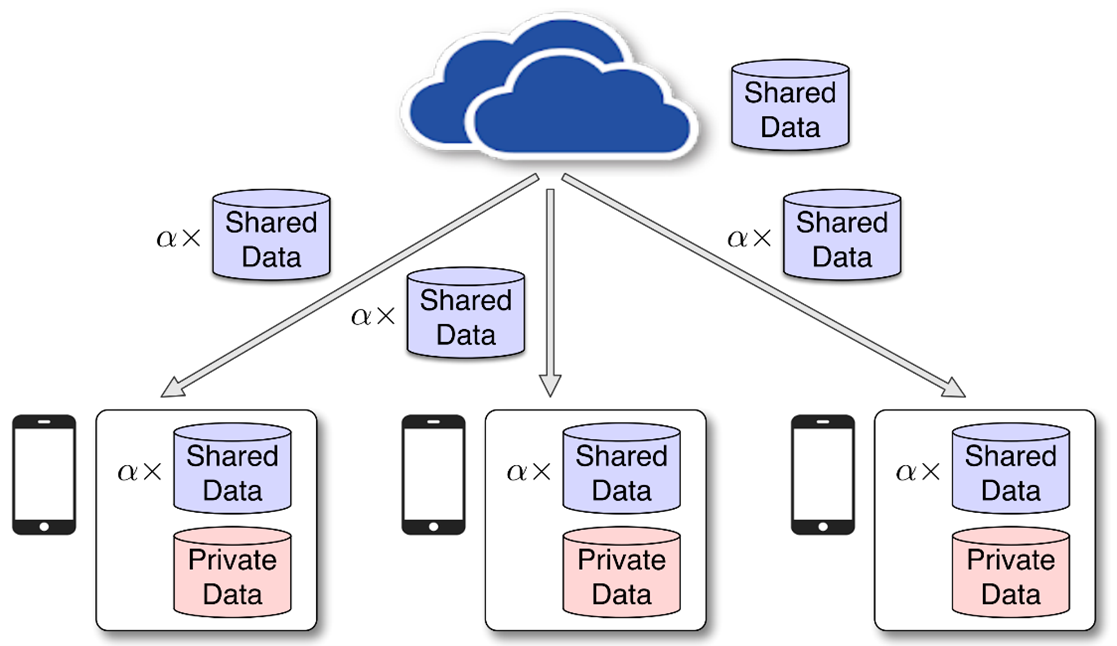
\includegraphics[scale=0.9]{images/chap3/share_data.png}%
	\caption{%
		نمایش نحوه به اشتراک‌ گذاری داده
		\cite{zhao2018federated}%
		.
	}
	\label{share_data}
	\centering
\end{figure}


\subsection{
	بهبود داده%
\protect
\LTRfootnote{Data Enhancement}
}
ابتدا، کاربران تعدادی از داده‌های خود را به سمت سرور ارسال می‌کنند. سرور، با استفاده از داده‌های دریافتی، یک مدل شبکه مولد رقابتی%
\LTRfootnote{Generative Adversarial Network (GAN)}
ایجاد می‌کند و این مدل را برای تمامی کاربران ارسال می‌نماید. کاربران با استفاده از این شبکه مولد رقابتی و با توجه به داده‌های خود، تعدادی داده جدید تولید کرده و در مراحل بعدی آموزش از این داده‌ها نیز استفاده می‌کنند. به این ترتیب، شبکه مولد رقابتی به کاربران کمک می‌کند تا داده‌های بیشتری برای آموزش مدل‌های خود در اختیار داشته باشند و از این داده‌ها برای بهبود عملکرد مدل‌های خود استفاده کنند.

در شکل
\ref{gan}%
نحوه عملکرد این روش به تصویر کشیده شده است. این روش، به دلیل استفاده از تکنیک‌های رمزگذاری%
\LTRfootnote{Encoding}
و رمزگشایی%
\LTRfootnote{Decoding}
داده‌ها، نسبت به روش‌های اشتراک‌گذاری داده‌ها از نظر حفظ حریم شخصی کاربران بهتر عمل می‌کند. به این معنی که، به جای ارسال داده‌های خام کاربران به سرور یا دیگر کاربران، از داده‌های تولید شده توسط شبکه مولد رقابتی استفاده می‌شود که احتمال نقض حریم شخصی را کاهش می‌دهد.

استفاده از تکنیک‌های رمزگذاری و رمزگشایی داده‌ها در این روش، باعث می‌شود که داده‌های حساس کاربران در طول فرآیند آموزش، به صورت امن باقی بمانند. به عبارت دیگر، حتی اگر داده‌ها در طول انتقال یا در سرور مورد دسترسی غیرمجاز قرار گیرند، به دلیل رمزگذاری، اطلاعات واقعی کاربران فاش نخواهد شد. این ویژگی، امنیت و حریم شخصی کاربران را به طور قابل توجهی افزایش می‌دهد و از اطلاعات حساس آنان در برابر تهدیدات محافظت می‌کند
\cite{jeong2018communication}.

بنابراین، روش‌های بهبود داده شده که مبتنی بر رمزگذاری و رمزگشایی داده‌ها هستند، نه تنها به بهبود عملکرد مدل‌های یادگیری کمک می‌کنند، بلکه از حریم شخصی کاربران نیز حفاظت می‌نمایند. این ترکیب از امنیت و کارایی، این روش‌ها را به گزینه‌های مناسبی برای استفاده در سیستم‌های یادگیری فدرال تبدیل کرده است.

\begin{figure}[t]
	\centering
	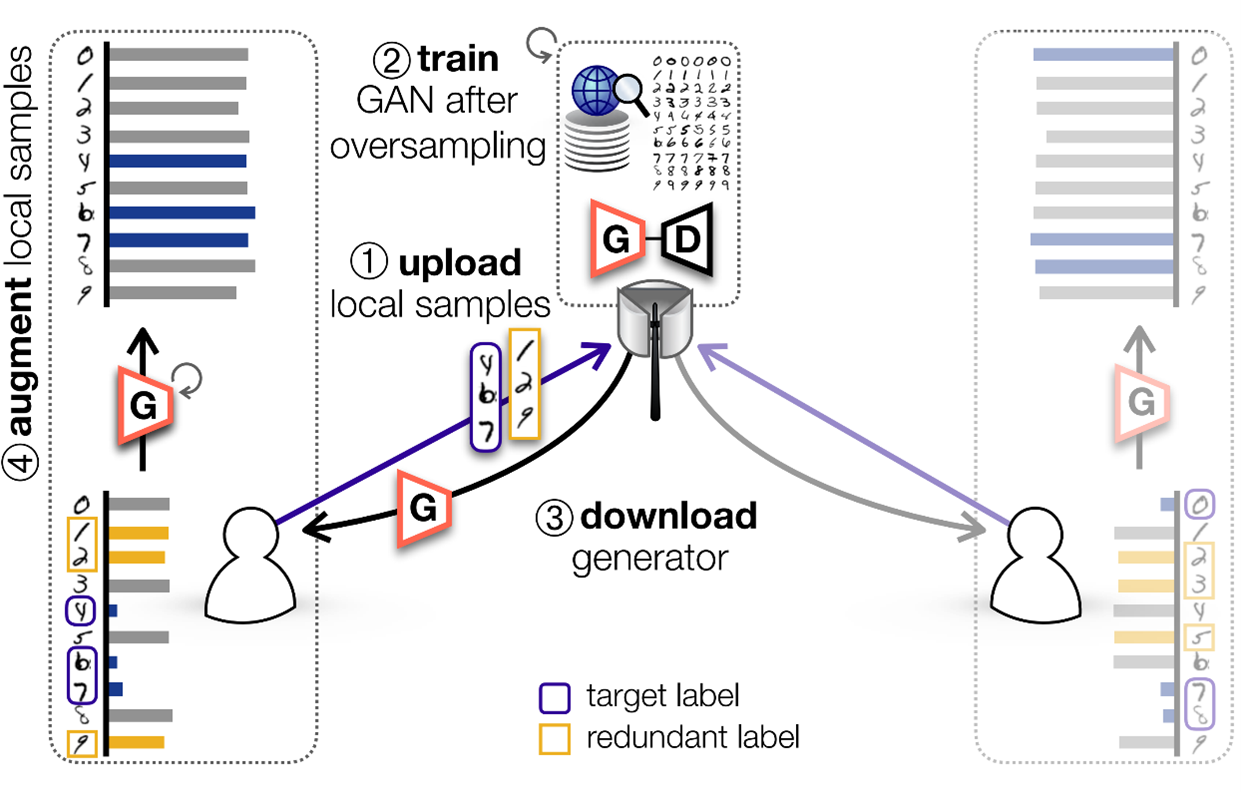
\includegraphics[scale=0.9]{images/chap3/generative_adversarial_network.png}%
	\caption{%
		استفاده از شبکه مولد رقابتی جهت تولید داده
		\cite{jeong2018communication}%
		.
	}
	\label{gan}
	\centering
\end{figure}


\subsection{انتخاب داده}
در هنگام انتخاب کاربران برای فرآیند آموزش، می‌توان از الگوریتم‌هایی که بر پایه کیفیت داده‌ها عمل می‌کنند، استفاده نمود. به عبارت دیگر، می‌توان از الگوریتم حریصانه کوله‌پشتی برای اولویت‌بندی کاربران بهره برد، به نحوی که کاربران با داده‌های غنی و گسترده‌تر، اولویت بالاتری جهت انتخاب داشته باشند. این رویکرد به بهبود کیفیت آموزش کمک می‌کند، زیرا داده‌های با کیفیت بالاتر تاثیر مثبتی بر نتایج نهایی مدل خواهند داشت
\cite{taik2021data}.

علاوه بر این، می‌توان از روش‌های یادگیری عمیق برای تخمین زمان اجرای مدل در سمت کاربران استفاده کرد. این روش‌ها می‌توانند زمان مورد نیاز برای اجرای مدل را پیش‌بینی کنند و بر اساس این پیش‌بینی، از بین ویژگی‌های مختلف جهت آموزش، تنها آن‌هایی را انتخاب نمایند که تاثیر بیشتری بر خروجی خواهند داشت. به این ترتیب، با بهینه‌سازی انتخاب ویژگی‌ها، می‌توان زمان و منابع محاسباتی را به شکل موثرتری مدیریت کرد.

یکی از نکات کلیدی در استفاده از این روش‌های انتخاب داده این است که هیچ کدام از آن‌ها تغییری بر روی داده‌ها و کاربران ایجاد نمی‌کنند. به عبارت دیگر، این روش‌ها به گونه‌ای طراحی شده‌اند که داده‌های موجود و وضعیت کاربران بدون تغییر باقی می‌مانند، اما فرآیند انتخاب و استفاده از داده‌ها بهینه‌تر و کارآمدتر می‌شود. این ویژگی، استفاده از این راه‌حل‌ها را در برنامه‌های مختلف بسیار کاربردی و موثر می‌سازد
\cite{zeng2022local}.

در نتیجه، استفاده از الگوریتم‌های مبتنی بر کیفیت داده‌ها و روش‌های یادگیری عمیق برای تخمین زمان اجرا، می‌تواند به طور قابل توجهی فرآیند آموزش در سیستم‌های یادگیری فدرال را بهبود بخشد. این روش‌ها نه تنها کیفیت داده‌های مورد استفاده را افزایش می‌دهند، بلکه با بهینه‌سازی منابع محاسباتی و زمان اجرا، کارایی سیستم را نیز بهبود می‌بخشند. این ترکیب از بهینه‌سازی داده‌ها و مدیریت منابع، به ویژه در محیط‌های با منابع محدود، اهمیت ویژه‌ای دارد و می‌تواند به نتایج بهتری در آموزش مدل‌ها منجر شود.





\section{نگرش برپایه چهارچوب}
تست


\section{نگرش برپایه الگوریتم}
تست
